\section{Πρωτόκολλα επικοινωνίας}
\label{sec:theory_protocols}

Τα \textit{Πρωτόκολλα επικοινωνίας} είναι ένα σύνολο κανόνων που επιτρέπουν σε δύο ή περισσότερα συστήματα επικοινωνίας να ανταλλάσουν δεδομένα μέσω οποιουδήποτε φυσικού μέσου. Οι κανόνες και ο συγχρονισμός μεταξύ των συστημάτων, η σύνταξη που πρέπει να ακολουθηθεί και η σημασιολογία ορίζονται όλα με τον όρο πρωτόκολλο. Τα πρωτόκολλα μπορούν να υλοποιηθούν τόσο από υλικό όσο και από λογισμκό ή από συνδυασμό και των δύο. Τα αναλογικά και ψηφιακά συστήματα επικοινωνίας χρησιμοποιούν ευρέως διαάφορα πρωτόκολλα επικοινωνίας. Επιπλέον κάθε πρωτόκολλο έχει τη δική του περιοχή εφαρμογής.

Στην περίπτωση του IoT, τα μέρη ενός συστήματος πρέπει να επικοινωνούν μεταξύ τους για να παρέχουν την αναμενόμενη έξοδο. Κάθε οντότητα θα πρέπει να συμφωνεί με κάποιο πρωτόκολλο για την ανταλλαγή πληροφοριών. Πολλά διαφορετικά πρωτόκολλα είναι διαθέσιμα για IoT συσκευές και αναπτύσσονται ανάλογα με την περιοχή εφαρμογής.

Στην παρούσα εργασία υποστηρίζονται τρία διαφορετικά πρωτόκολλα επικοινωνίας, τα οποία παρουσιάζονται παρακάτω.

\subsection{I2C}
\label{subsec:i2c}

Το \textit{Inter Intergrated Circuit} (\textit{I2C}) είναι ένα σειριακό πρωτόκολλο επικοινωνίας το οποίο αναπτύχθηκε από την Philips Semiconductors\footnote{\url{https://www.nxp.com/}}. Ο κύριος σκοπός του είναι να παρέχει ευκολία στη σύνδεση περιφερειακών τσιπ με μικροελεγκτή. 

Είναι master-slave (αφέντης-σκλάβος) πρωτόκολλο επικοινωνίας. Κάθε slave έχει μια μοναδική διεύθυνση. Για να επιτευχθεί η επικοινωνία, η master συσκευή αρχικά αποστέλλει την διεύθυνση του επιθυμητού slave μαζί με τη σημαία R/W (read/write ή ανάγνωση/εγγραφή). Η αντίστοιχη slave συσκευή θα μεταβεί σε ενεργή λειτουργία.

Εφόσον η slave συσκευή είναι έτοιμη, ξεκινάει η επικοινωνία μεταξύ master και slave. Για να λειτουργήσει χρειάζεται δύο διαύλους, το SDA και το SCL, όπως φαίνεται και στο \autoref{fig:i2c}.

\begin{figure}[!ht]
	\centering
	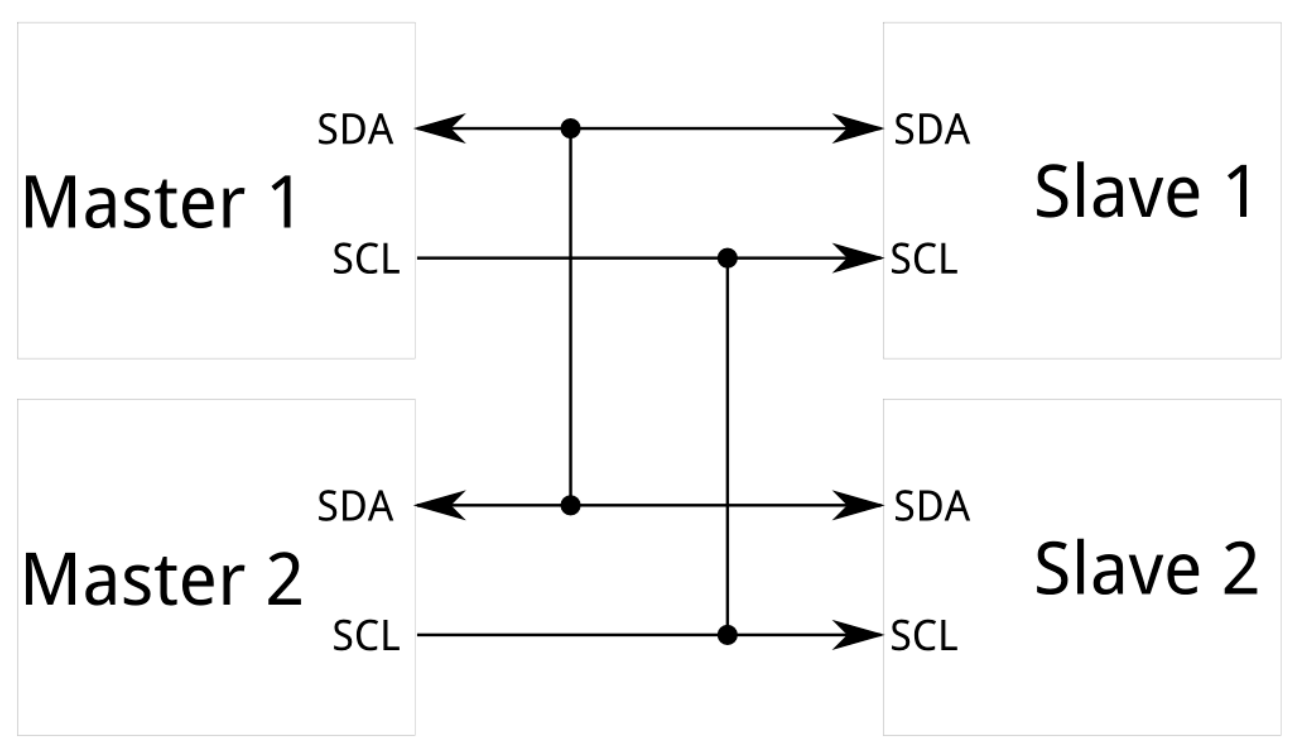
\includegraphics[width=0.6\textwidth]{./images/chapter2/i2c.png}
	\caption{I2C}
	\label{fig:i2c}
\end{figure}

\subsection{SPI}
\label{subsec:SPI}

Το \textit{Serial Peripheral Interface} (\textit{SPI}) αναπτύχθηκε από τη Motorola\footnote{\url{https://www.motorola.com/us/}} και αποτελείται από τους ακόλουθους διαύλους:

\begin{itemize}
	\item MOSI: Master Out Slave in
	\item MISO: Master In Slave Out
	\item SS: Slave Select
	\item SCLK: Serial Clock
	\item Ακριβής χρονισμός
\end{itemize}

Μια αναπαράσταση των διαύλων μπορούμε να δούμε στο \autoref{fig:spi}. Όπως το I2C, έτσι και το SPI είναι πρωτόκολλο επικοινωνίας master-slave. Στο SPI, πρώτα η master συσκευή διαμορφώνει το ρολόι σε μια συγκεκριμένη συχνότητα. Επιπλέον ο δίαυλος SS χρησιμοποιείται για την επιλογή του κατάλληλου slave. Αφού επιλεγεί η slave συσκευή, αρχίζει η επικοινωνία.

\begin{figure}[!ht]
	\centering
	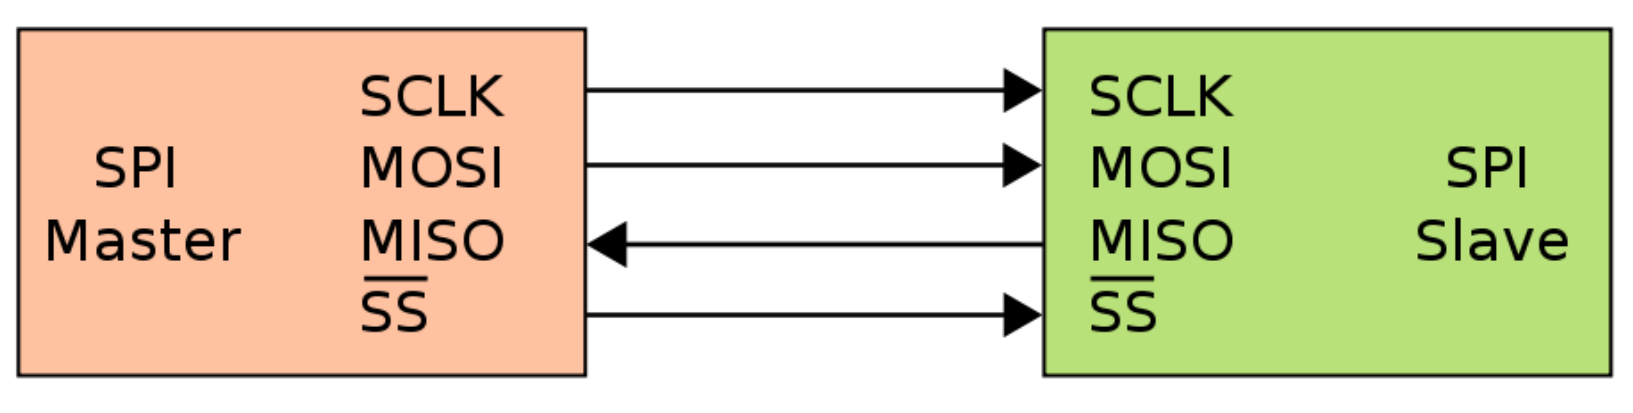
\includegraphics[width=0.8\textwidth]{./images/chapter2/spi.png}
	\caption{SPI}
	\label{fig:spi}
\end{figure}

\subsection{UART}
\label{subsec:UART}

Το \textit{Universal Asynchronous Receiver/Transmitter} (\textit{UART}) δεν είναι ακριβώς πρωτόκολλο αλλά ένα φυσικό κομμάτι υλικού που μετατρέπει παράλληλα δεδομένα σε σειρειακά. Ο κύριος σκοπός του είναι η μετάδοση και λήψη δεδομένων σειριακά.

Αποτελείται από δύο διαύλους έναν για την αποστολή των δεδομένων και έναν για τη λήψη. Επομένως χρειάζεται δύο ακροδέκτες, ο Rx (δέκτης) και ο Tx (πομπός), το οποίο φαίνεται και στο \autoref{fig:uart}).

Το UART μεταδίδει δεδομένα ασύγχρονα, άρα κάνενα σήμα ρολογιού δεν σχετίζεται με τη μετάδοση και τη λήψη δεδομένων. Αντί για σήμα ρολογιού, χρησιμοποιεί bit έναρξης και διακοπής μέσω πραγματικών bit δεδομένων, τα οποία καθορίζουν την έναρξη και το τέλος του πακέτου δεδομένων.

\begin{figure}[!ht]
	\centering
	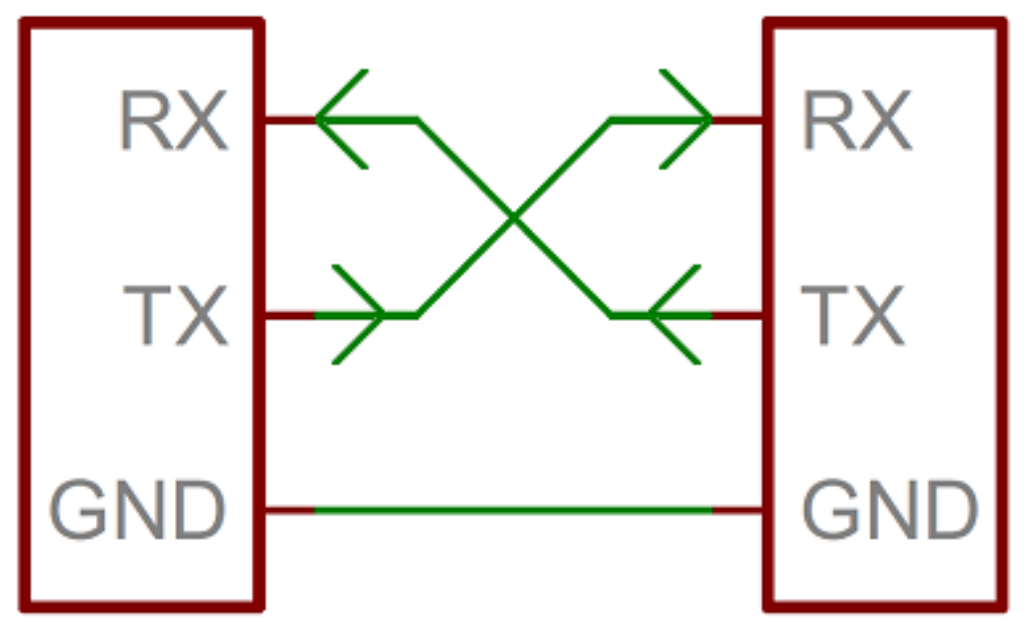
\includegraphics[width=0.5\textwidth]{./images/chapter2/uart.png}
	\caption{UART}
	\label{fig:uart}
\end{figure}